\documentclass[11pt]{article}
\usepackage[margin=0.8in,landscape]{geometry}
\usepackage{booktabs}
\usepackage[dvipsnames]{xcolor}
\usepackage{amsmath}
\usepackage{amssymb}
\usepackage{graphicx}
\newcommand{\finding}[1]{\par\medskip\noindent\fcolorbox{black!30}{yellow!10}{\parbox{0.97\textwidth}{\textbf{Findings.} #1}}\medskip}

\title{Heteroscedastic mixed-variable BO benchmark --- progress report}
\author{}
\date{July 22, 2026}

\begin{document}
\maketitle

\section{Scope and status of the runs}

The benchmark compares \textbf{4 surrogate models} (Separate GP, Categorical-kernel GP,
Standard LVGP, Heteroscedastic LVGP) $\times$ \textbf{6 acquisitions} (EI/LCB/PI +
noise-aware HAEI/ANPEI/RAHBO) $\times$ $n_{\mathrm{rep}}\in\{3,10\}$ replicates $\times$
5 seeds on 9 mixed-variable heteroscedastic test problems (200 BO iterations for the
multi-dimensional problems, 50 for the 1-D ones; shared SLHD initial designs per seed ---
common random numbers across all models). The sweep runs python models first, all
$n_{\mathrm{rep}}{=}10$ blocks before $n_{\mathrm{rep}}{=}3$, and the 10-D problem last.

\begin{table}[h]
\centering\small
\begin{tabular}{lrl}
\toprule
Problem & Complete & Note \\
\midrule
ackley\_2d, branin\_hetero, griewank\_2d, sixhump\_camel & 100\% & 1-D; also carry the full 30-seed evidence from the earlier sweep \\
otl\_circuit, piston, rastrigin\_6d & 100\% & multi-dimensional (d = 5--6) \\
golinski & 97\% & 6 cells lost to an early 8\,h timeout (since raised to 16\,h); refill pass pending \\
ackley\_10d & 32\% & \emph{in progress} --- heter-LVGP cells still pending \\
\bottomrule
\end{tabular}
\caption{Run status as of July 22, 2026 (sweep position 1748/2100 grid cells).}
\end{table}

\section{Computational cost and the 5-seed decision}

\begin{table}[h]
\centering\small
\begin{tabular}{lrrrr}
\toprule
 & Separate GP & Categorical kernel & Standard LVGP & Heteroscedastic LVGP \\
\midrule
1-D problems (50 iter)        & 18--44\,s   & 54--114\,s  & 5--11\,min      & 5--13\,min \\
d = 5--6 problems (200 iter)  & 20--40\,min & 43--110\,min & 4.3--7.3\,h    & 4.6--6.9\,h \\
ackley\_10d (200 iter)        & 1.1\,h      & 3.2\,h      & \textbf{20.1\,h} & pending (projected $\sim$1--1.5\,d) \\
\bottomrule
\end{tabular}
\caption{Measured mean wall-clock per cell (one full BO run). The MATLAB LVGP engines cost
$\sim$10--25$\times$ the python GP models; the validated native python LVGP port
(\texttt{compare\_matlab\_python.ipynb}) is the mitigation path for the 10-D block.}
\end{table}

\paragraph{Why 5 seeds.}
The sweep runs 24 parallel workers on the shared node, so the constraint is total compute, not
sequential time: at the measured per-cell costs the full 30-seed grid amounts to roughly
$3\times10^4$ core-hours (dominated by the MATLAB LVGPs on the $d\ge5$ problems and the 10-D
block), i.e.\ $\approx$7--8 \emph{weeks} of wall-clock even at full 24-way parallelism ---
monopolizing a node shared with other users. Five seeds with both $n_{\mathrm{rep}}$ cut this
to $\approx$9 days of wall-clock (consistent with the observed pace: $\sim$85\% of the grid
in 6 days) while still populating \emph{every} (model, acquisition, problem) cell,
seed-paired across models via the shared initial designs. The
analysis compensates statistically (medians/IQR, cross-problem rank consistency rather than
per-problem significance), the four 1-D problems retain their 30-seed evidence, and the
harness is resumable so seeds can be extended selectively later.

\clearpage
\section{Regret convergence}

\begin{figure}[h]
\centering
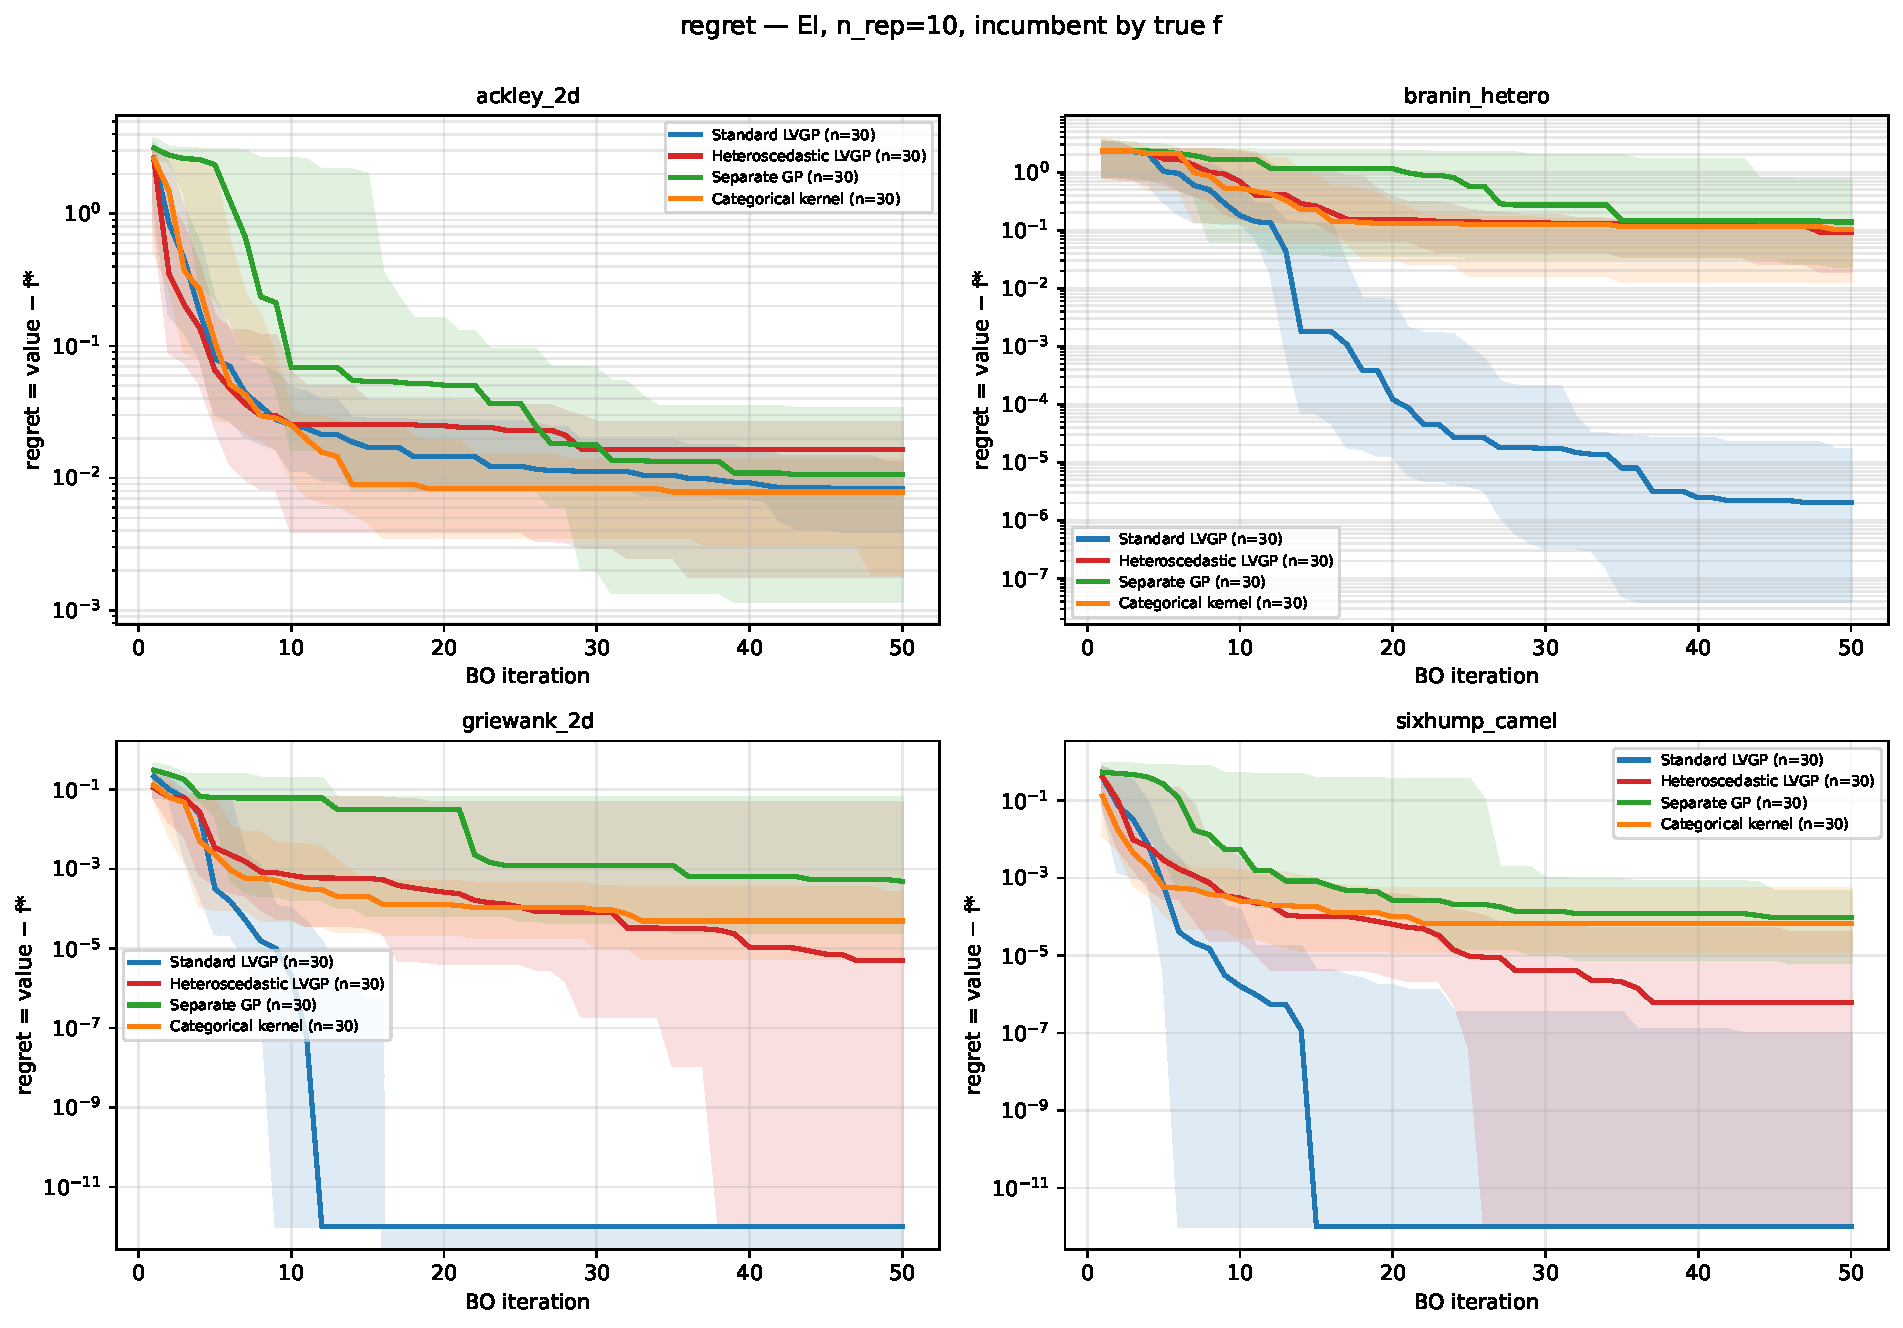
\includegraphics[height=0.80\textheight]{figs/regret_conv_1d.pdf}
\caption{Regret convergence (EI, $n_{\mathrm{rep}}=10$, median $\pm$ IQR over seeds) --- 1-D
problems. Other acquisitions: \texttt{compare.ipynb} Part~3/6.}
\end{figure}

\clearpage
\begin{figure}[h]
\centering
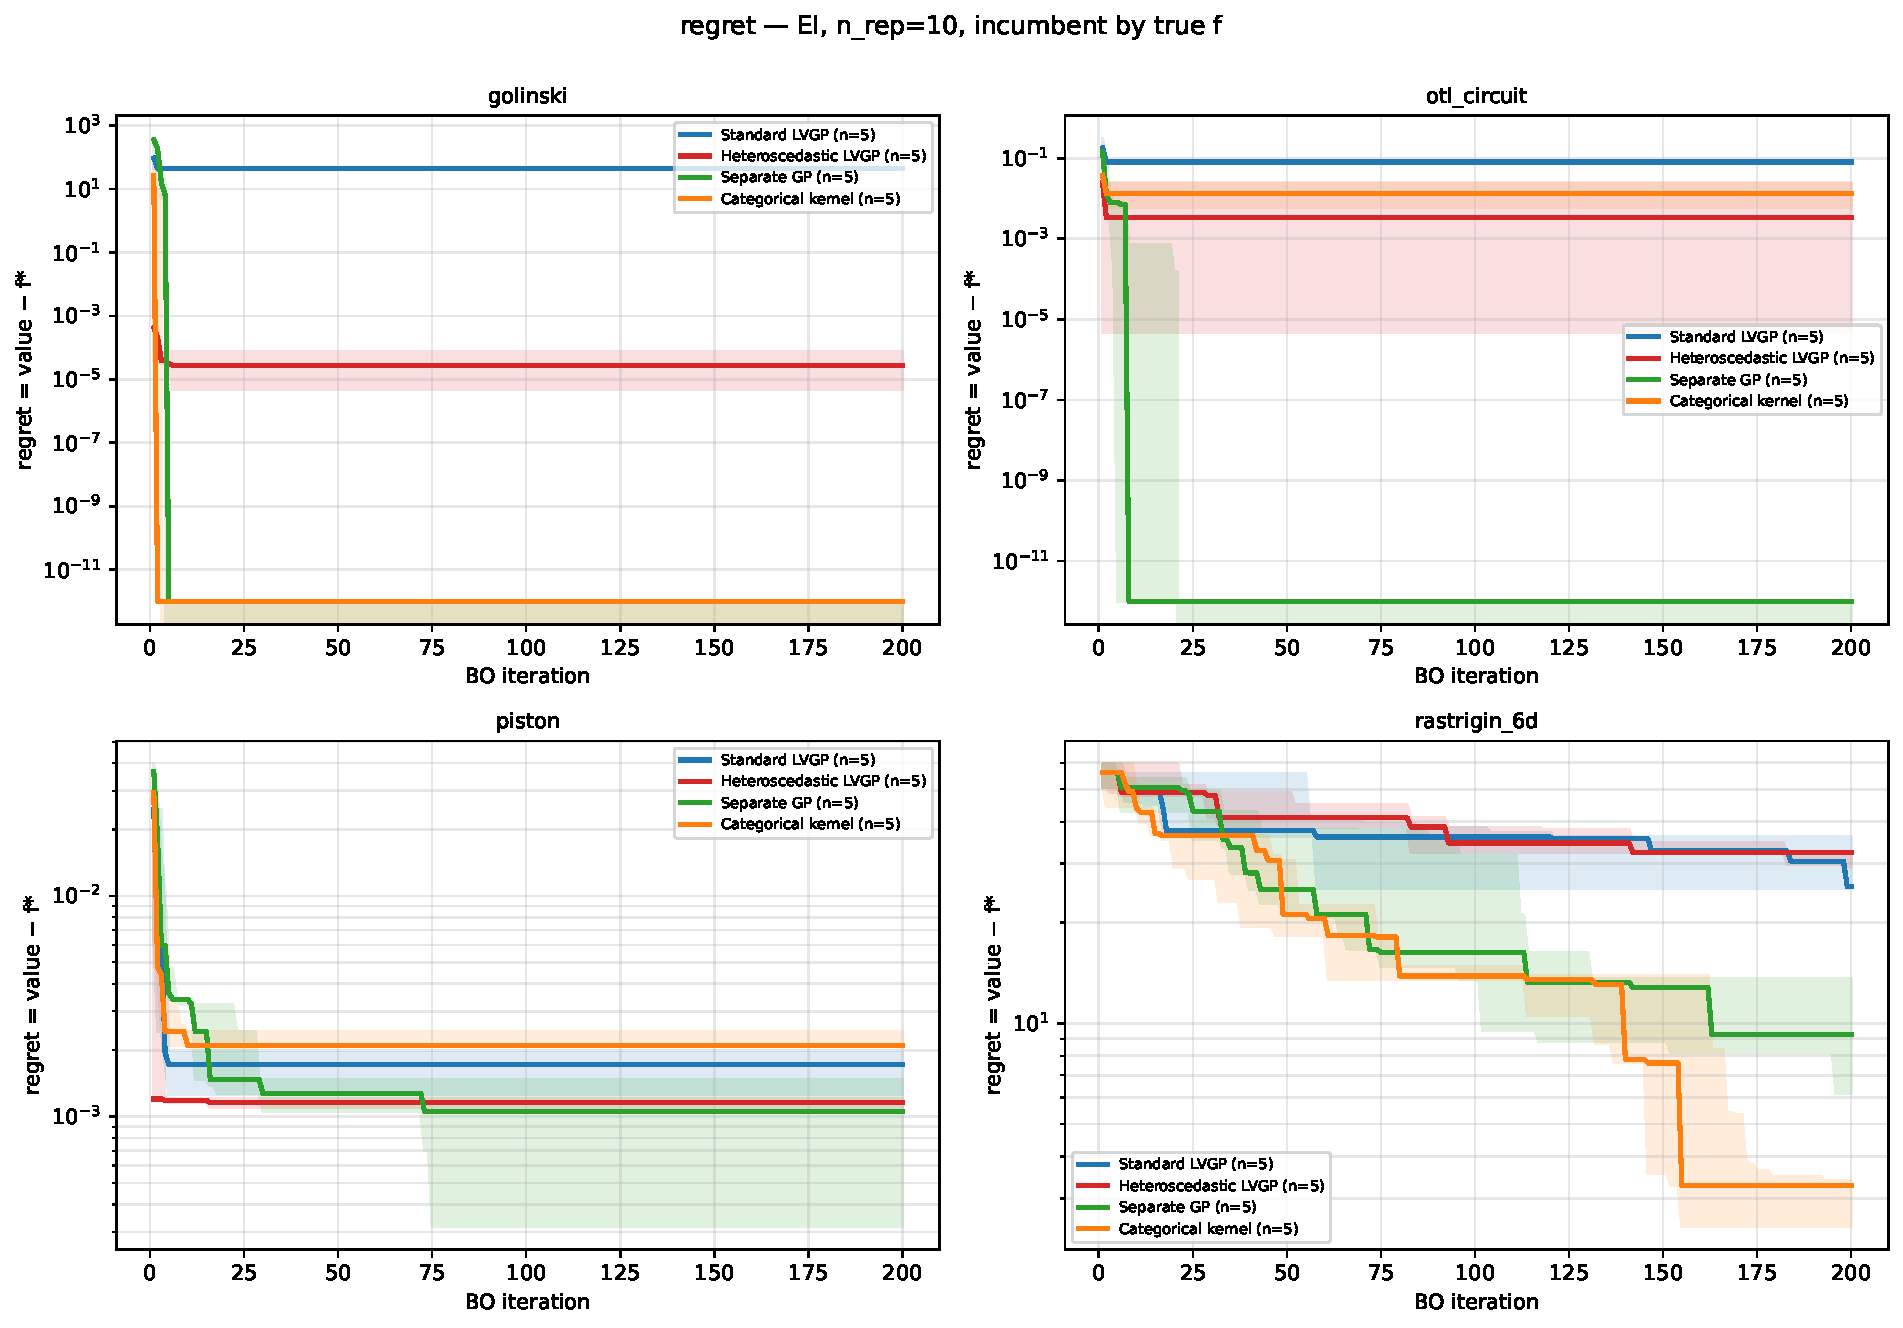
\includegraphics[height=0.66\textheight]{figs/regret_conv_md.pdf}
\caption{Regret convergence (EI, $n_{\mathrm{rep}}=10$) --- multi-dimensional problems.}
\end{figure}

\finding{
(1) On the 1-D problems every model converges to the optimum region; the MATLAB LVGPs
exploit it tightest --- note this partly reflects their BO loop, not only the model (verified:
the loop effect appears for non-LVGP models too), so cross-engine regret gaps should be read
with care.
(2) \textbf{golinski exposes noise-blindness}: the Standard LVGP's median final regret under
EI is $\approx 44$ (PI: $\approx 49$) while the heteroscedastic LVGP and both python GPs
solve the problem to $\approx 0$ --- the optimum sits in a region with replicate variance
$\sigma^2 = 576$, and fitting replicate means as if noiseless breaks the model there.
(3) \textbf{rastrigin\_6d is the hardest problem so far} and is led by the python GPs
(median EI regret: categorical $3.3$, separate $9.3$) with both LVGPs trailing (standard
$25.6$, heter $32.3$) --- surface accuracy dominates on this rugged landscape.
(4) otl\_circuit and piston are near-solved by all models (regret $\le 0.08$); differences
there are in \emph{design noise}, not in $f$ (see \S5--6).}

\clearpage
\section{Final regret tables}
\noindent\textbf{Legend (all tables).} Cell = final metric (mean $\pm$ sd over seeds).
\textbf{Bold} = best model for that acquisition; \colorbox{green!20}{green} = best
(acquisition, model) combination for that problem. Lower is better.

\input{regret_nrep10_1d.tex}
\clearpage
\begin{table}[htbp]
\centering
\small
\setlength{\tabcolsep}{4pt}
\setlength{\fboxsep}{2pt}
\caption{Final regret (value $-$ $f^*$) for every acquisition $\times$ surrogate model ($n_{\mathrm{rep}}=10$, mean $\pm$ sd over seeds).}
\label{tab:regret_nrep10}
\begin{tabular}{llrrrr}
\toprule
Acquisition & Model & Golinski & OTL Circuit & Piston & Rastrigin 6-D \\
\midrule
LCB & Standard LVGP & $2.5{\times}10^{-6} \pm 8.5{\times}10^{-8}$ & $3.87{\times}10^{-6} \pm 3.2{\times}10^{-6}$ & \colorbox{green!20}{{\boldmath$2.16{\times}10^{-7} \pm 1.5{\times}10^{-7}$}} & $28.3 \pm 6.1$ \\
 & Heteroscedastic LVGP & $1.26{\times}10^{-7} \pm 1.3{\times}10^{-9}$ & $4.64{\times}10^{-7} \pm 3.8{\times}10^{-7}$ & $4.62{\times}10^{-7} \pm 5.1{\times}10^{-7}$ & $25 \pm 5.7$ \\
 & Separate GP & \colorbox{green!20}{{\boldmath$0 \pm 0$}} & $0.00142 \pm 0.0028$ & $0.00104 \pm 0.00071$ & $18.2 \pm 9.6$ \\
 & Categorical kernel & \colorbox{green!20}{{\boldmath$0 \pm 0$}} & \colorbox{green!20}{{\boldmath$0 \pm 0$}} & $0.00105 \pm 0.00023$ & {\boldmath$6.49 \pm 4.2$} \\
\midrule
PI & Standard LVGP & $43.8 \pm 0$ & $0.055 \pm 0.03$ & $0.00127 \pm 0.00052$ & $20.7 \pm 6.8$ \\
 & Heteroscedastic LVGP & $1.37 \pm 2.6$ & $0.00558 \pm 0.0096$ & {\boldmath$2.93{\times}10^{-5} \pm 3.7{\times}10^{-5}$} & $23.4 \pm 3.2$ \\
 & Separate GP & \colorbox{green!20}{{\boldmath$0 \pm 0$}} & {\boldmath$6.94{\times}10^{-5} \pm 7{\times}10^{-5}$} & $0.000532 \pm 0.00038$ & $13.6 \pm 3.8$ \\
 & Categorical kernel & \colorbox{green!20}{{\boldmath$0 \pm 0$}} & $0.0158 \pm 0.011$ & $0.00125 \pm 0.0011$ & \colorbox{green!20}{{\boldmath$3.87 \pm 2.8$}} \\
\midrule
EI & Standard LVGP & $37.3 \pm 13$ & $0.0659 \pm 0.03$ & $0.0025 \pm 0.0021$ & $30.6 \pm 9.4$ \\
 & Heteroscedastic LVGP & $6.39{\times}10^{-5} \pm 7.9{\times}10^{-5}$ & $0.0121 \pm 0.014$ & $0.00109 \pm 0.0006$ & $31.2 \pm 2.5$ \\
 & Separate GP & \colorbox{green!20}{{\boldmath$0 \pm 0$}} & {\boldmath$3.07{\times}10^{-5} \pm 6.1{\times}10^{-5}$} & {\boldmath$0.001 \pm 0.00074$} & $12.2 \pm 8$ \\
 & Categorical kernel & \colorbox{green!20}{{\boldmath$0 \pm 0$}} & $0.0163 \pm 0.014$ & $0.00205 \pm 0.00054$ & {\boldmath$3.89 \pm 2.2$} \\
\midrule
HAEI ($\gamma=0.5$) & Heteroscedastic LVGP & $7.82 \pm 4.1$ & $0.0117 \pm 0.013$ & $0.00336 \pm 0.0018$ & $30.4 \pm 4.9$ \\
 & Separate GP & \colorbox{green!20}{{\boldmath$0 \pm 0$}} & {\boldmath$3.07{\times}10^{-5} \pm 6.1{\times}10^{-5}$} & {\boldmath$0.000822 \pm 0.00057$} & $9.46 \pm 2.4$ \\
 & Categorical kernel & \colorbox{green!20}{{\boldmath$0 \pm 0$}} & $0.0155 \pm 0.013$ & $0.0026 \pm 0.00096$ & {\boldmath$4.8 \pm 1.6$} \\
\midrule
ANPEI ($\beta=0.8$) & Heteroscedastic LVGP & $0.965 \pm 1.4$ & $0.0039 \pm 0.0073$ & {\boldmath$0.00173 \pm 0.0013$} & $24.3 \pm 5.9$ \\
 & Separate GP & \colorbox{green!20}{{\boldmath$0 \pm 0$}} & {\boldmath$0.000162 \pm 0.00029$} & $0.00209 \pm 0.0007$ & $12.6 \pm 3.4$ \\
 & Categorical kernel & \colorbox{green!20}{{\boldmath$0 \pm 0$}} & $0.0287 \pm 0.017$ & $0.00238 \pm 0.0008$ & {\boldmath$3.95 \pm 2$} \\
\midrule
RAHBO ($\alpha=0.5$) & Heteroscedastic LVGP & {\boldmath$2.44 \pm 2.5$} & $2.74{\times}10^{-7} \pm 1.7{\times}10^{-7}$ & {\boldmath$4.58{\times}10^{-7} \pm 5.5{\times}10^{-7}$} & $20.5 \pm 4.5$ \\
 & Separate GP & $17.5 \pm 28$ & $0.00142 \pm 0.0028$ & $0.00123 \pm 0.00062$ & $20.4 \pm 7.4$ \\
 & Categorical kernel & $10.6 \pm 4$ & \colorbox{green!20}{{\boldmath$0 \pm 0$}} & $0.000715 \pm 0.00033$ & {\boldmath$5.19 \pm 2.6$} \\
\bottomrule
\end{tabular}
\end{table}

\clearpage
\input{regret_nrep03_1d.tex}
\clearpage
\begin{table}[htbp]
\centering
\small
\setlength{\tabcolsep}{4pt}
\setlength{\fboxsep}{2pt}
\caption{Final regret (value $-$ $f^*$) for every acquisition $\times$ surrogate model ($n_{\mathrm{rep}}=3$, mean $\pm$ sd over seeds).}
\label{tab:regret_nrep03}
\begin{tabular}{llrrrr}
\toprule
Acquisition & Model & Golinski & OTL Circuit & Piston & Rastrigin 6-D \\
\midrule
LCB & Standard LVGP & $2.56{\times}10^{-6} \pm 8.5{\times}10^{-8}$ & $1.53{\times}10^{-6} \pm 9.7{\times}10^{-7}$ & $0.000307 \pm 0.00029$ & $23.5 \pm 8.7$ \\
 & Heteroscedastic LVGP & $1.24{\times}10^{-7} \pm 1{\times}10^{-8}$ & \colorbox{green!20}{{\boldmath$4.33{\times}10^{-7} \pm 5.5{\times}10^{-7}$}} & \colorbox{green!20}{{\boldmath$1.49{\times}10^{-6} \pm 1.5{\times}10^{-6}$}} & $22.7 \pm 6.9$ \\
 & Separate GP & \colorbox{green!20}{{\boldmath$0 \pm 0$}} & $0.00142 \pm 0.0028$ & $0.0011 \pm 0.0007$ & $18.9 \pm 8.3$ \\
 & Categorical kernel & \colorbox{green!20}{{\boldmath$0 \pm 0$}} & $3.07{\times}10^{-5} \pm 6.1{\times}10^{-5}$ & $0.000715 \pm 0.00033$ & {\boldmath$7.57 \pm 4.4$} \\
\midrule
PI & Standard LVGP & $31.6 \pm 17$ & $0.0242 \pm 0.022$ & $0.00168 \pm 0.001$ & $11.6 \pm 3.7$ \\
 & Heteroscedastic LVGP & $0.941 \pm 1.9$ & $0.00164 \pm 0.0012$ & {\boldmath$0.000361 \pm 0.0004$} & $19.1 \pm 2.4$ \\
 & Separate GP & \colorbox{green!20}{{\boldmath$0 \pm 0$}} & {\boldmath$1.74{\times}10^{-5} \pm 2.3{\times}10^{-5}$} & $0.000718 \pm 0.00046$ & $17.2 \pm 6.5$ \\
 & Categorical kernel & \colorbox{green!20}{{\boldmath$0 \pm 0$}} & $0.0155 \pm 0.011$ & $0.00177 \pm 0.00093$ & \colorbox{green!20}{{\boldmath$4.18 \pm 3.2$}} \\
\midrule
EI & Standard LVGP & $16.3 \pm 17$ & $0.0565 \pm 0.02$ & $0.00339 \pm 0.0033$ & $19.5 \pm 12$ \\
 & Heteroscedastic LVGP & $0.000119 \pm 0.00015$ & $0.0119 \pm 0.013$ & $0.00182 \pm 0.0015$ & $24.4 \pm 8.1$ \\
 & Separate GP & \colorbox{green!20}{{\boldmath$0 \pm 0$}} & {\boldmath$0.00033 \pm 0.00041$} & {\boldmath$0.00131 \pm 0.00074$} & $15.1 \pm 8.4$ \\
 & Categorical kernel & \colorbox{green!20}{{\boldmath$0 \pm 0$}} & $0.0218 \pm 0.018$ & $0.00267 \pm 0.00088$ & {\boldmath$5.61 \pm 3.9$} \\
\midrule
HAEI ($\gamma=0.5$) & Heteroscedastic LVGP & $3.75 \pm 2.1$ & $0.0268 \pm 0.029$ & $0.00197 \pm 0.0013$ & $28.1 \pm 8.4$ \\
 & Separate GP & \colorbox{green!20}{{\boldmath$0 \pm 0$}} & {\boldmath$0.000173 \pm 0.00028$} & {\boldmath$0.00163 \pm 0.00073$} & $9.95 \pm 3.9$ \\
 & Categorical kernel & \colorbox{green!20}{{\boldmath$0 \pm 0$}} & $0.0203 \pm 0.017$ & $0.00189 \pm 0.00073$ & {\boldmath$4.92 \pm 1.7$} \\
\midrule
ANPEI ($\beta=0.8$) & Heteroscedastic LVGP & $0.307 \pm 0.61$ & $0.0147 \pm 0.012$ & {\boldmath$0.00246 \pm 0.0012$} & $26.3 \pm 5.6$ \\
 & Separate GP & \colorbox{green!20}{{\boldmath$0 \pm 0$}} & {\boldmath$0.000322 \pm 0.0004$} & $0.00254 \pm 0.00099$ & $11.2 \pm 4.1$ \\
 & Categorical kernel & $1.49 \pm 3$ & $0.0146 \pm 0.013$ & $0.00295 \pm 0.0018$ & {\boldmath$7.34 \pm 5.3$} \\
\midrule
RAHBO ($\alpha=0.5$) & Heteroscedastic LVGP & {\boldmath$9.65 \pm 6.6$} & {\boldmath$6.33{\times}10^{-7} \pm 4.8{\times}10^{-7}$} & {\boldmath$1.71{\times}10^{-6} \pm 3{\times}10^{-6}$} & $22.4 \pm 8.3$ \\
 & Separate GP & $56.7 \pm 47$ & $0.00142 \pm 0.0028$ & $0.00112 \pm 0.00073$ & $20.1 \pm 10$ \\
 & Categorical kernel & $20 \pm 29$ & $1.23{\times}10^{-5} \pm 2.5{\times}10^{-5}$ & $0.000713 \pm 0.00054$ & {\boldmath$8.7 \pm 4.2$} \\
\bottomrule
\end{tabular}
\end{table}


\finding{
(1) $n_{\mathrm{rep}}=10$ vs $3$: more replicates help the noise-aware configurations most
(their noise estimates stabilize); the ranking of models is broadly stable across both.
(2) The best single configurations per problem (green cells) are spread across models ---
no single (model, acquisition) wins everywhere; the heteroscedastic LVGP collects its wins
on the problems where noise matters (golinski, otl, piston), the categorical GP on the
rugged rastrigin.}

\clearpage
\section{Noise at the incumbent (lower = quieter design)}
\input{noise_nrep10_1d.tex}
\clearpage
\begin{table}[htbp]
\centering
\small
\setlength{\tabcolsep}{4pt}
\setlength{\fboxsep}{2pt}
\caption{Final noise $\sigma^2$ at the incumbent design for every acquisition $\times$ surrogate model ($n_{\mathrm{rep}}=10$, mean $\pm$ sd over seeds).}
\label{tab:noise_nrep10}
\begin{tabular}{llrrrr}
\toprule
Acquisition & Model & Golinski & OTL Circuit & Piston & Rastrigin 6-D \\
\midrule
LCB & Standard LVGP & $576 \pm 3.9{\times}10^{-8}$ & $0.000194 \pm 1.4{\times}10^{-10}$ & $0.000256 \pm 7.3{\times}10^{-10}$ & $1.97 \pm 1.3$ \\
 & Heteroscedastic LVGP & $576 \pm 5.2{\times}10^{-10}$ & $0.000194 \pm 2.7{\times}10^{-11}$ & $0.000256 \pm 1.7{\times}10^{-9}$ & $1.24 \pm 0.13$ \\
 & Separate GP & \colorbox{green!20}{{\boldmath$576 \pm 0$}} & $0.000651 \pm 0.00091$ & {\boldmath$0.000195 \pm 5.7{\times}10^{-5}$} & $2.11 \pm 2$ \\
 & Categorical kernel & \colorbox{green!20}{{\boldmath$576 \pm 0$}} & \colorbox{green!20}{{\boldmath$0.000194 \pm 0$}} & $0.000234 \pm 5{\times}10^{-6}$ & {\boldmath$1.15 \pm 0.079$} \\
\midrule
PI & Standard LVGP & $605 \pm 0$ & $0.00121 \pm 0.00064$ & $0.000211 \pm 3.9{\times}10^{-5}$ & $1.16 \pm 0.044$ \\
 & Heteroscedastic LVGP & $576 \pm 0.0015$ & $0.000474 \pm 0.00034$ & $0.000256 \pm 5.3{\times}10^{-10}$ & $1.85 \pm 1.5$ \\
 & Separate GP & \colorbox{green!20}{{\boldmath$576 \pm 0$}} & \colorbox{green!20}{{\boldmath$0.000194 \pm 0$}} & $0.000241 \pm 8.8{\times}10^{-6}$ & $1.14 \pm 0.054$ \\
 & Categorical kernel & \colorbox{green!20}{{\boldmath$576 \pm 0$}} & $0.000333 \pm 0.00028$ & {\boldmath$0.000197 \pm 5.6{\times}10^{-5}$} & {\boldmath$1.11 \pm 0.04$} \\
\midrule
EI & Standard LVGP & $602 \pm 6.2$ & $0.000886 \pm 3.6{\times}10^{-6}$ & {\boldmath$0.000159 \pm 5.3{\times}10^{-5}$} & $2.97 \pm 2$ \\
 & Heteroscedastic LVGP & $576 \pm 3.9{\times}10^{-6}$ & $0.000474 \pm 0.00034$ & $0.000233 \pm 4.7{\times}10^{-5}$ & $1.28 \pm 0.16$ \\
 & Separate GP & \colorbox{green!20}{{\boldmath$576 \pm 0$}} & \colorbox{green!20}{{\boldmath$0.000194 \pm 0$}} & $0.000241 \pm 8.8{\times}10^{-6}$ & $1.97 \pm 1.7$ \\
 & Categorical kernel & \colorbox{green!20}{{\boldmath$576 \pm 0$}} & $0.000235 \pm 8.1{\times}10^{-5}$ & $0.000203 \pm 3.6{\times}10^{-5}$ & {\boldmath$1.12 \pm 0.043$} \\
\midrule
HAEI ($\gamma=0.5$) & Heteroscedastic LVGP & $576 \pm 7.1{\times}10^{-6}$ & $0.000474 \pm 0.00034$ & \colorbox{green!20}{{\boldmath$0.000124 \pm 5.3{\times}10^{-5}$}} & $1.3 \pm 0.15$ \\
 & Separate GP & \colorbox{green!20}{{\boldmath$576 \pm 0$}} & \colorbox{green!20}{{\boldmath$0.000194 \pm 0$}} & $0.000225 \pm 3.5{\times}10^{-5}$ & \colorbox{green!20}{{\boldmath$1.07 \pm 0.077$}} \\
 & Categorical kernel & \colorbox{green!20}{{\boldmath$576 \pm 0$}} & $0.000413 \pm 0.00025$ & $0.000142 \pm 6.1{\times}10^{-5}$ & $1.09 \pm 0.041$ \\
\midrule
ANPEI ($\beta=0.8$) & Heteroscedastic LVGP & $576 \pm 5.7{\times}10^{-6}$ & $0.000375 \pm 0.00027$ & $0.000175 \pm 7.4{\times}10^{-5}$ & $1.12 \pm 0.12$ \\
 & Separate GP & \colorbox{green!20}{{\boldmath$576 \pm 0$}} & {\boldmath$0.000235 \pm 8.1{\times}10^{-5}$} & $0.000199 \pm 4.4{\times}10^{-5}$ & $1.17 \pm 0.11$ \\
 & Categorical kernel & \colorbox{green!20}{{\boldmath$576 \pm 0$}} & $0.000377 \pm 0.00027$ & {\boldmath$0.000137 \pm 2.7{\times}10^{-5}$} & {\boldmath$1.1 \pm 0.031$} \\
\midrule
RAHBO ($\alpha=0.5$) & Heteroscedastic LVGP & $576 \pm 0.74$ & $0.000194 \pm 1.1{\times}10^{-11}$ & $0.000256 \pm 6.6{\times}10^{-10}$ & $1.26 \pm 0.073$ \\
 & Separate GP & $589 \pm 25$ & $0.000651 \pm 0.00091$ & {\boldmath$0.000178 \pm 5.2{\times}10^{-5}$} & $1.9 \pm 1.4$ \\
 & Categorical kernel & \colorbox{green!20}{{\boldmath$576 \pm 0$}} & \colorbox{green!20}{{\boldmath$0.000194 \pm 0$}} & $0.000236 \pm 6.2{\times}10^{-6}$ & {\boldmath$1.11 \pm 0.044$} \\
\bottomrule
\end{tabular}
\end{table}

\clearpage
\input{noise_nrep03_1d.tex}
\clearpage
\begin{table}[htbp]
\centering
\small
\setlength{\tabcolsep}{4pt}
\setlength{\fboxsep}{2pt}
\caption{Final noise $\sigma^2$ at the incumbent design for every acquisition $\times$ surrogate model ($n_{\mathrm{rep}}=3$, mean $\pm$ sd over seeds).}
\label{tab:noise_nrep03}
\begin{tabular}{llrrrr}
\toprule
Acquisition & Model & Golinski & OTL Circuit & Piston & Rastrigin 6-D \\
\midrule
LCB & Standard LVGP & $576 \pm 3.9{\times}10^{-8}$ & $0.000194 \pm 5.3{\times}10^{-11}$ & $0.000247 \pm 7.7{\times}10^{-6}$ & $1.28 \pm 0.12$ \\
 & Heteroscedastic LVGP & $576 \pm 4.9{\times}10^{-9}$ & $0.000194 \pm 1.7{\times}10^{-11}$ & $0.000256 \pm 7.3{\times}10^{-9}$ & $1.29 \pm 0.12$ \\
 & Separate GP & \colorbox{green!20}{{\boldmath$576 \pm 0$}} & $0.000651 \pm 0.00091$ & {\boldmath$0.000183 \pm 5.8{\times}10^{-5}$} & $2.68 \pm 1.9$ \\
 & Categorical kernel & \colorbox{green!20}{{\boldmath$576 \pm 0$}} & \colorbox{green!20}{{\boldmath$0.000194 \pm 0$}} & $0.000236 \pm 6.2{\times}10^{-6}$ & {\boldmath$1.13 \pm 0.044$} \\
\midrule
PI & Standard LVGP & $597 \pm 19$ & $0.000753 \pm 0.00028$ & {\boldmath$0.000196 \pm 5{\times}10^{-5}$} & {\boldmath$1.13 \pm 0.089$} \\
 & Heteroscedastic LVGP & $576 \pm 4{\times}10^{-5}$ & $0.000514 \pm 0.00032$ & $0.000256 \pm 4.3{\times}10^{-9}$ & $1.26 \pm 0.1$ \\
 & Separate GP & \colorbox{green!20}{{\boldmath$576 \pm 0$}} & \colorbox{green!20}{{\boldmath$0.000194 \pm 0$}} & $0.00021 \pm 4.2{\times}10^{-5}$ & $1.87 \pm 1.5$ \\
 & Categorical kernel & \colorbox{green!20}{{\boldmath$576 \pm 0$}} & $0.000908 \pm 0.0008$ & $0.000202 \pm 6.4{\times}10^{-5}$ & $1.15 \pm 0.091$ \\
\midrule
EI & Standard LVGP & $584 \pm 11$ & $0.00079 \pm 0.0002$ & $0.000175 \pm 3.7{\times}10^{-5}$ & $1.95 \pm 1.5$ \\
 & Heteroscedastic LVGP & $576 \pm 4{\times}10^{-6}$ & $0.000514 \pm 0.00032$ & $0.000223 \pm 5.7{\times}10^{-5}$ & $1.24 \pm 0.089$ \\
 & Separate GP & \colorbox{green!20}{{\boldmath$576 \pm 0$}} & {\boldmath$0.000275 \pm 9.9{\times}10^{-5}$} & $0.000209 \pm 5.3{\times}10^{-5}$ & $2.49 \pm 1.7$ \\
 & Categorical kernel & \colorbox{green!20}{{\boldmath$576 \pm 0$}} & $0.000514 \pm 0.00032$ & {\boldmath$0.000173 \pm 6.4{\times}10^{-5}$} & {\boldmath$1.11 \pm 0.037$} \\
\midrule
HAEI ($\gamma=0.5$) & Heteroscedastic LVGP & $576 \pm 9.1{\times}10^{-6}$ & $0.000512 \pm 0.00032$ & $0.000185 \pm 7.3{\times}10^{-5}$ & $1.3 \pm 0.21$ \\
 & Separate GP & \colorbox{green!20}{{\boldmath$576 \pm 0$}} & {\boldmath$0.000235 \pm 8.1{\times}10^{-5}$} & $0.000211 \pm 3.7{\times}10^{-5}$ & $1.19 \pm 0.1$ \\
 & Categorical kernel & \colorbox{green!20}{{\boldmath$576 \pm 0$}} & $0.000275 \pm 0.0001$ & {\boldmath$0.000185 \pm 6.9{\times}10^{-5}$} & {\boldmath$1.11 \pm 0.054$} \\
\midrule
ANPEI ($\beta=0.8$) & Heteroscedastic LVGP & $576 \pm 0.00033$ & $0.000275 \pm 9.9{\times}10^{-5}$ & \colorbox{green!20}{{\boldmath$0.00015 \pm 6.6{\times}10^{-5}$}} & \colorbox{green!20}{{\boldmath$1.09 \pm 0.041$}} \\
 & Separate GP & \colorbox{green!20}{{\boldmath$576 \pm 0$}} & {\boldmath$0.000275 \pm 9.9{\times}10^{-5}$} & $0.000161 \pm 7.4{\times}10^{-5}$ & $1.11 \pm 0.048$ \\
 & Categorical kernel & \colorbox{green!20}{{\boldmath$576 \pm 0$}} & $0.000333 \pm 0.00028$ & $0.000153 \pm 5.9{\times}10^{-5}$ & $1.1 \pm 0.027$ \\
\midrule
RAHBO ($\alpha=0.5$) & Heteroscedastic LVGP & {\boldmath$576 \pm 2.9{\times}10^{-6}$} & $0.000194 \pm 2.8{\times}10^{-11}$ & $0.000256 \pm 2.4{\times}10^{-8}$ & $1.25 \pm 0.1$ \\
 & Separate GP & $592 \pm 26$ & $0.000651 \pm 0.00091$ & {\boldmath$0.000198 \pm 5.8{\times}10^{-5}$} & $2.69 \pm 1.9$ \\
 & Categorical kernel & $587 \pm 22$ & \colorbox{green!20}{{\boldmath$0.000194 \pm 0$}} & $0.000231 \pm 3.8{\times}10^{-5}$ & {\boldmath$1.18 \pm 0.088$} \\
\bottomrule
\end{tabular}
\end{table}


\finding{
(1) On otl\_circuit all models reach top-tier $f$, but ranked against the whole design
space the heteroscedastic LVGP's noise-aware recommendations come from the \textbf{quietest
11\%} of designs vs.\ 34\% for both python GPs (percentile framing, \texttt{compare.ipynb}
Part~6) --- equal performance, $\sim$3$\times$ quieter design.
(2) On rastrigin the incumbent noise ordering is categorical $1.11$ $<$ separate $1.15$ $<$
heter $1.28$ --- where the heter LVGP's $f$-surface is weak, its noise advantage does not
compensate.
(3) On the 1-D problems the noise columns mostly mirror which minimum was found (quiet vs
noisy twin) --- the discriminating robustness view is \S6.}

\clearpage
\section{Heatmaps --- acquisition $\times$ model (multi-dimensional problems)}

\begin{figure}[h]
\centering
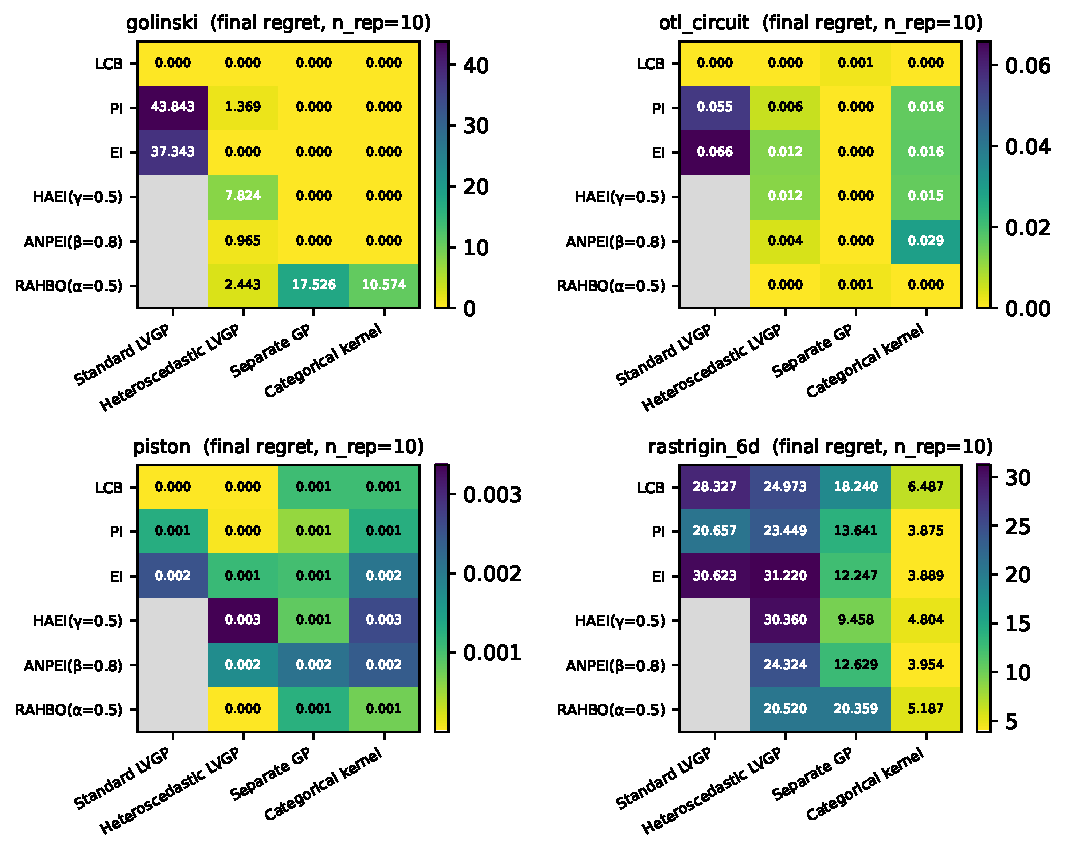
\includegraphics[width=0.8\textwidth]{figs/heatmaps_multidim_nrep10.pdf}
\caption{Final regret per acquisition $\times$ model for the multi-dimensional problems
($n_{\mathrm{rep}}=10$) --- the regime where regret is informative. Per-problem versions for
the 1-D problems: \texttt{compare.ipynb} Part~4.}
\end{figure}

\finding{
Reading the four panels column-wise: the Standard LVGP column is the weakest on golinski
(noise-blindness, cf.\ \S3) and rastrigin; the heteroscedastic LVGP column is strong on
golinski/otl/piston across acquisitions; the categorical GP dominates rastrigin under every
acquisition. Acquisition-wise, EI/LCB are the most reliable columns overall; PI is the most
erratic.}

\clearpage
\section{Work in progress --- mean--variance (MV) robustness}

Robustness is scored on the true $\mathrm{MV}_\alpha = f + \alpha\sigma^2$ of the recommended
design. Ground truth first: the MV optimum \emph{relocates to a different categorical level}
on branin ($\alpha\gtrsim7$), griewank\_2d ($\alpha\gtrsim13$) and golinski
($\alpha\gtrsim5$) --- the ``trap'' problems; camel and ackley are controls whose nominal
optima are already quiet. The current sweep runs RAHBO at $\alpha=0.5$ (below every
threshold), so the $\alpha\in\{1,5,15\}$ sensitivity sweep and a reporting-rule refinement
(\texttt{notes/README.md}) are pending before conclusions; tables below use $\alpha=1$.

\begin{figure}[h]
\centering
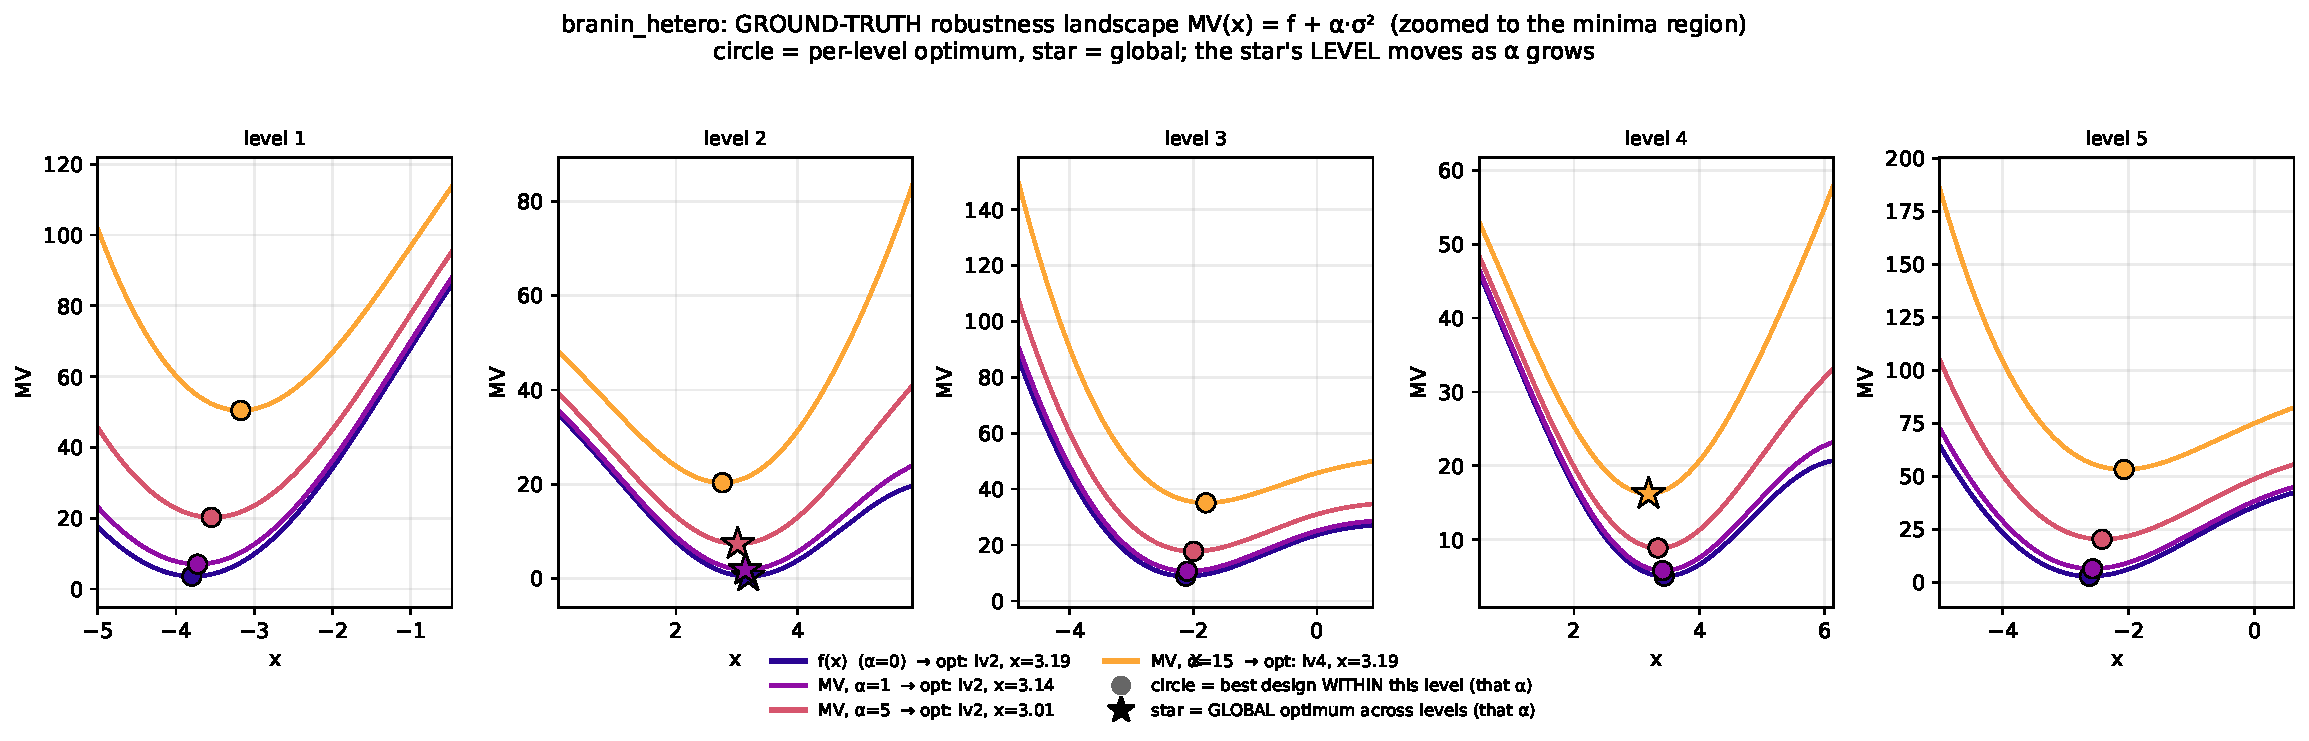
\includegraphics[width=0.72\textwidth]{figs/mv_landscape_branin_hetero.pdf}
\caption{Ground-truth MV landscape, \textbf{branin} (trap): the global optimum (star) moves
from level 2 to level 4 as $\alpha$ grows.}
\end{figure}

\clearpage
\begin{figure}[h]
\centering
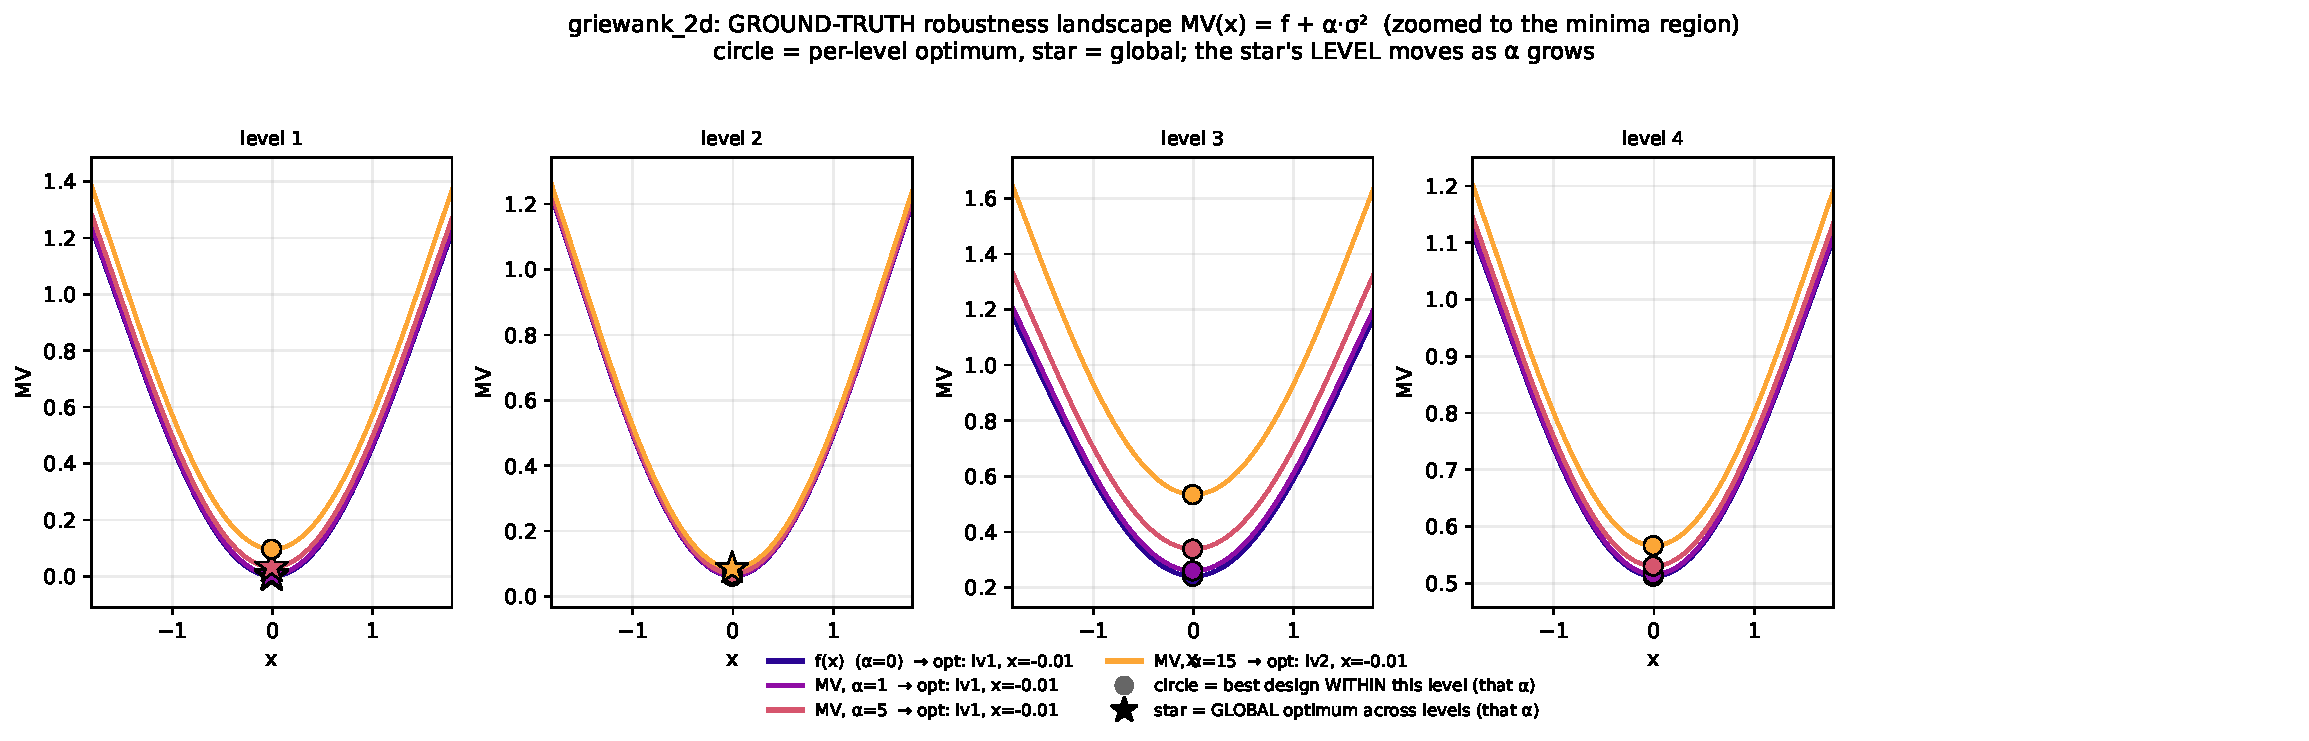
\includegraphics[width=0.72\textwidth]{figs/mv_landscape_griewank_2d.pdf}
\caption{Ground-truth MV landscape, \textbf{griewank\_2d} (trap at $\alpha\gtrsim13$:
level 1 $\to$ 2).}
\end{figure}

\clearpage
\begin{figure}[h]
\centering
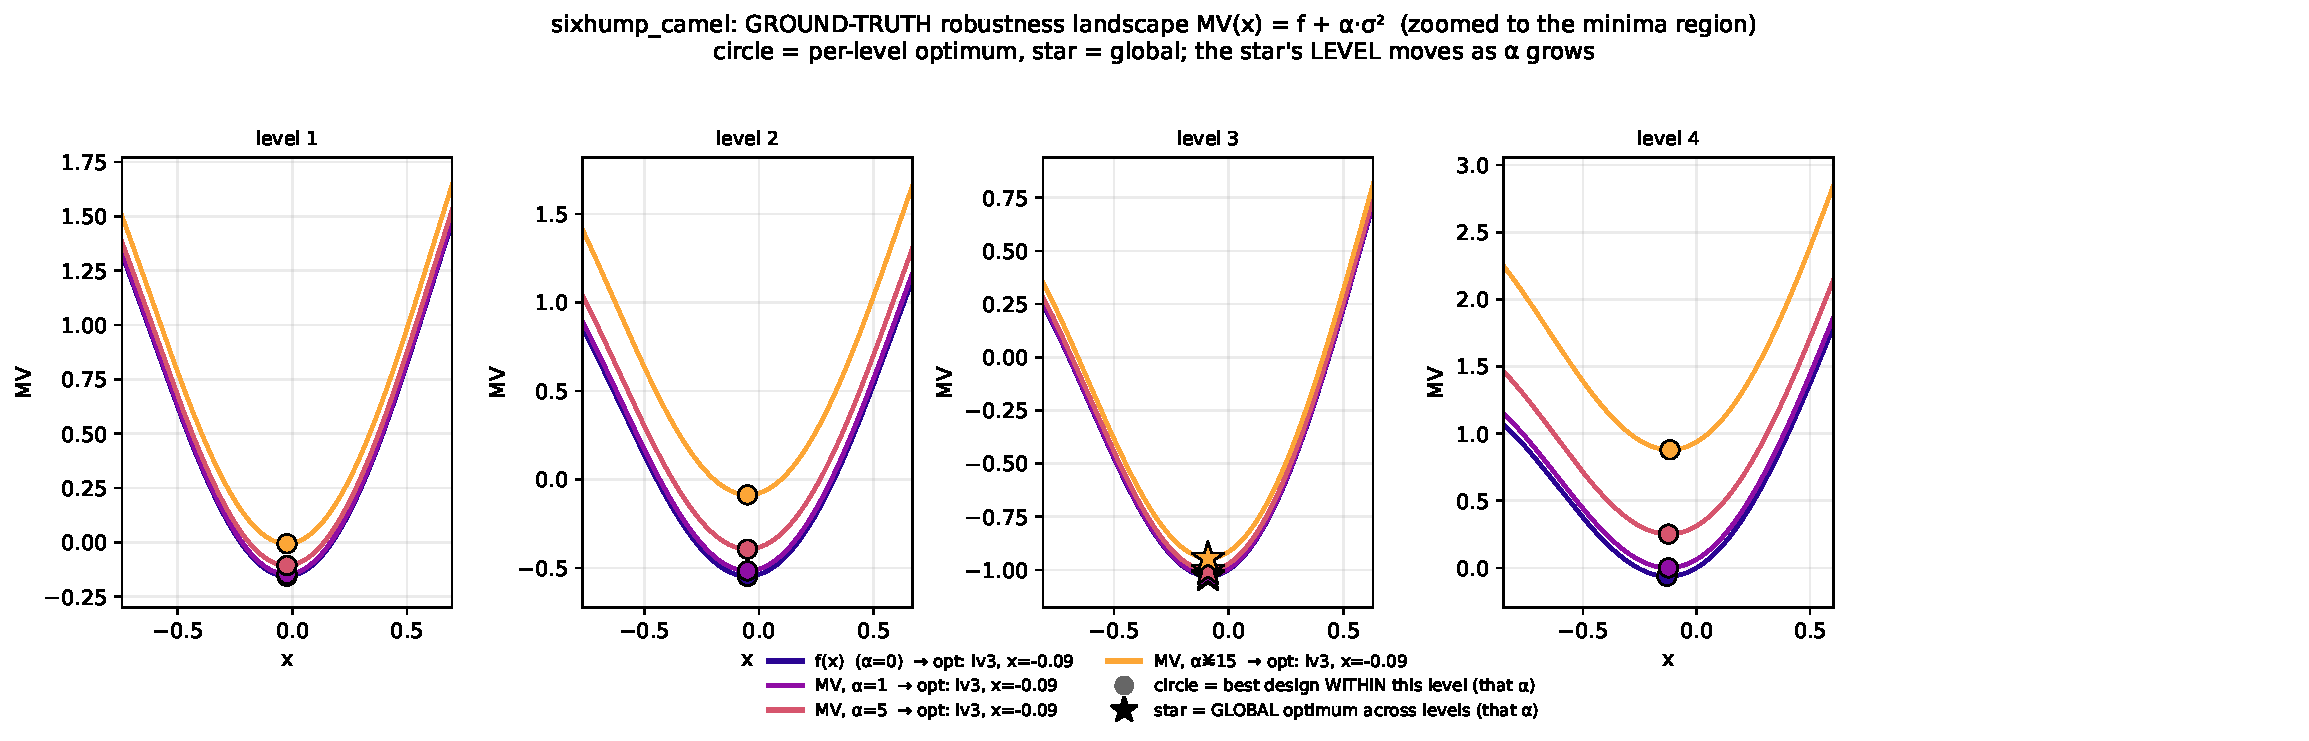
\includegraphics[width=0.72\textwidth]{figs/mv_landscape_sixhump_camel.pdf}
\caption{Ground-truth MV landscape, \textbf{sixhump\_camel} (control: the optimum never
moves --- already quiet).}
\end{figure}

\clearpage
\begin{figure}[h]
\centering
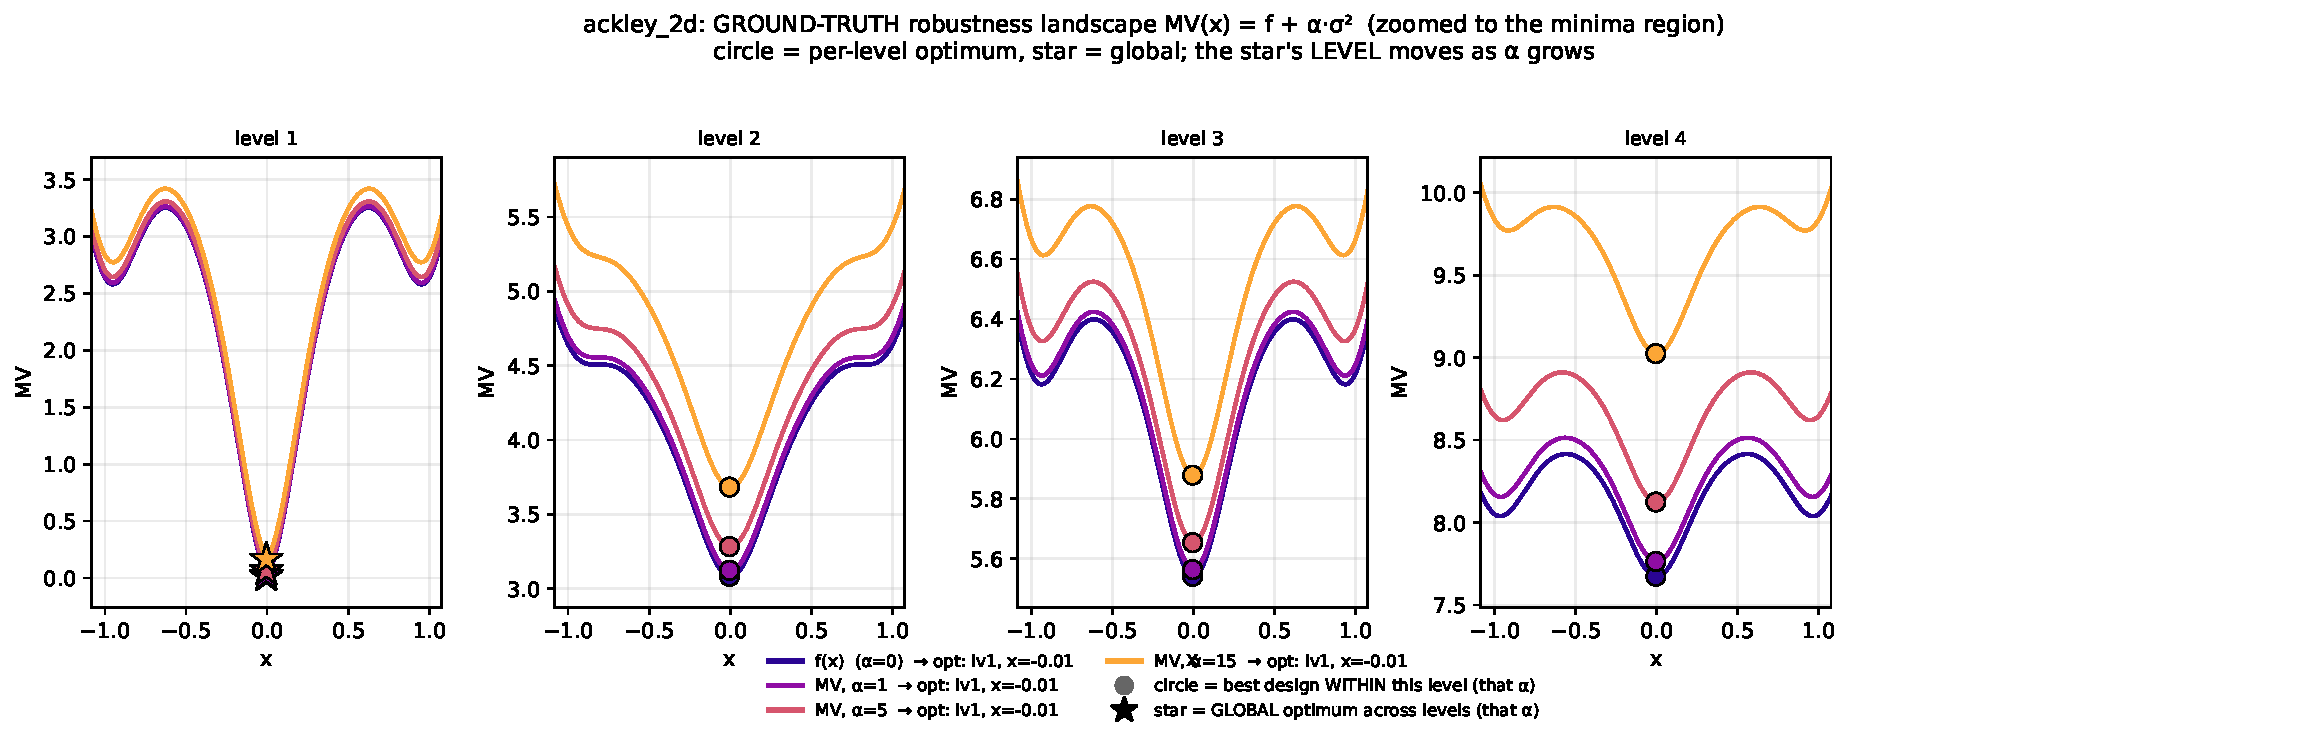
\includegraphics[width=0.72\textwidth]{figs/mv_landscape_ackley_2d.pdf}
\caption{Ground-truth MV landscape, \textbf{ackley\_2d} (control).}
\end{figure}

\clearpage
\begin{figure}[h]
\centering
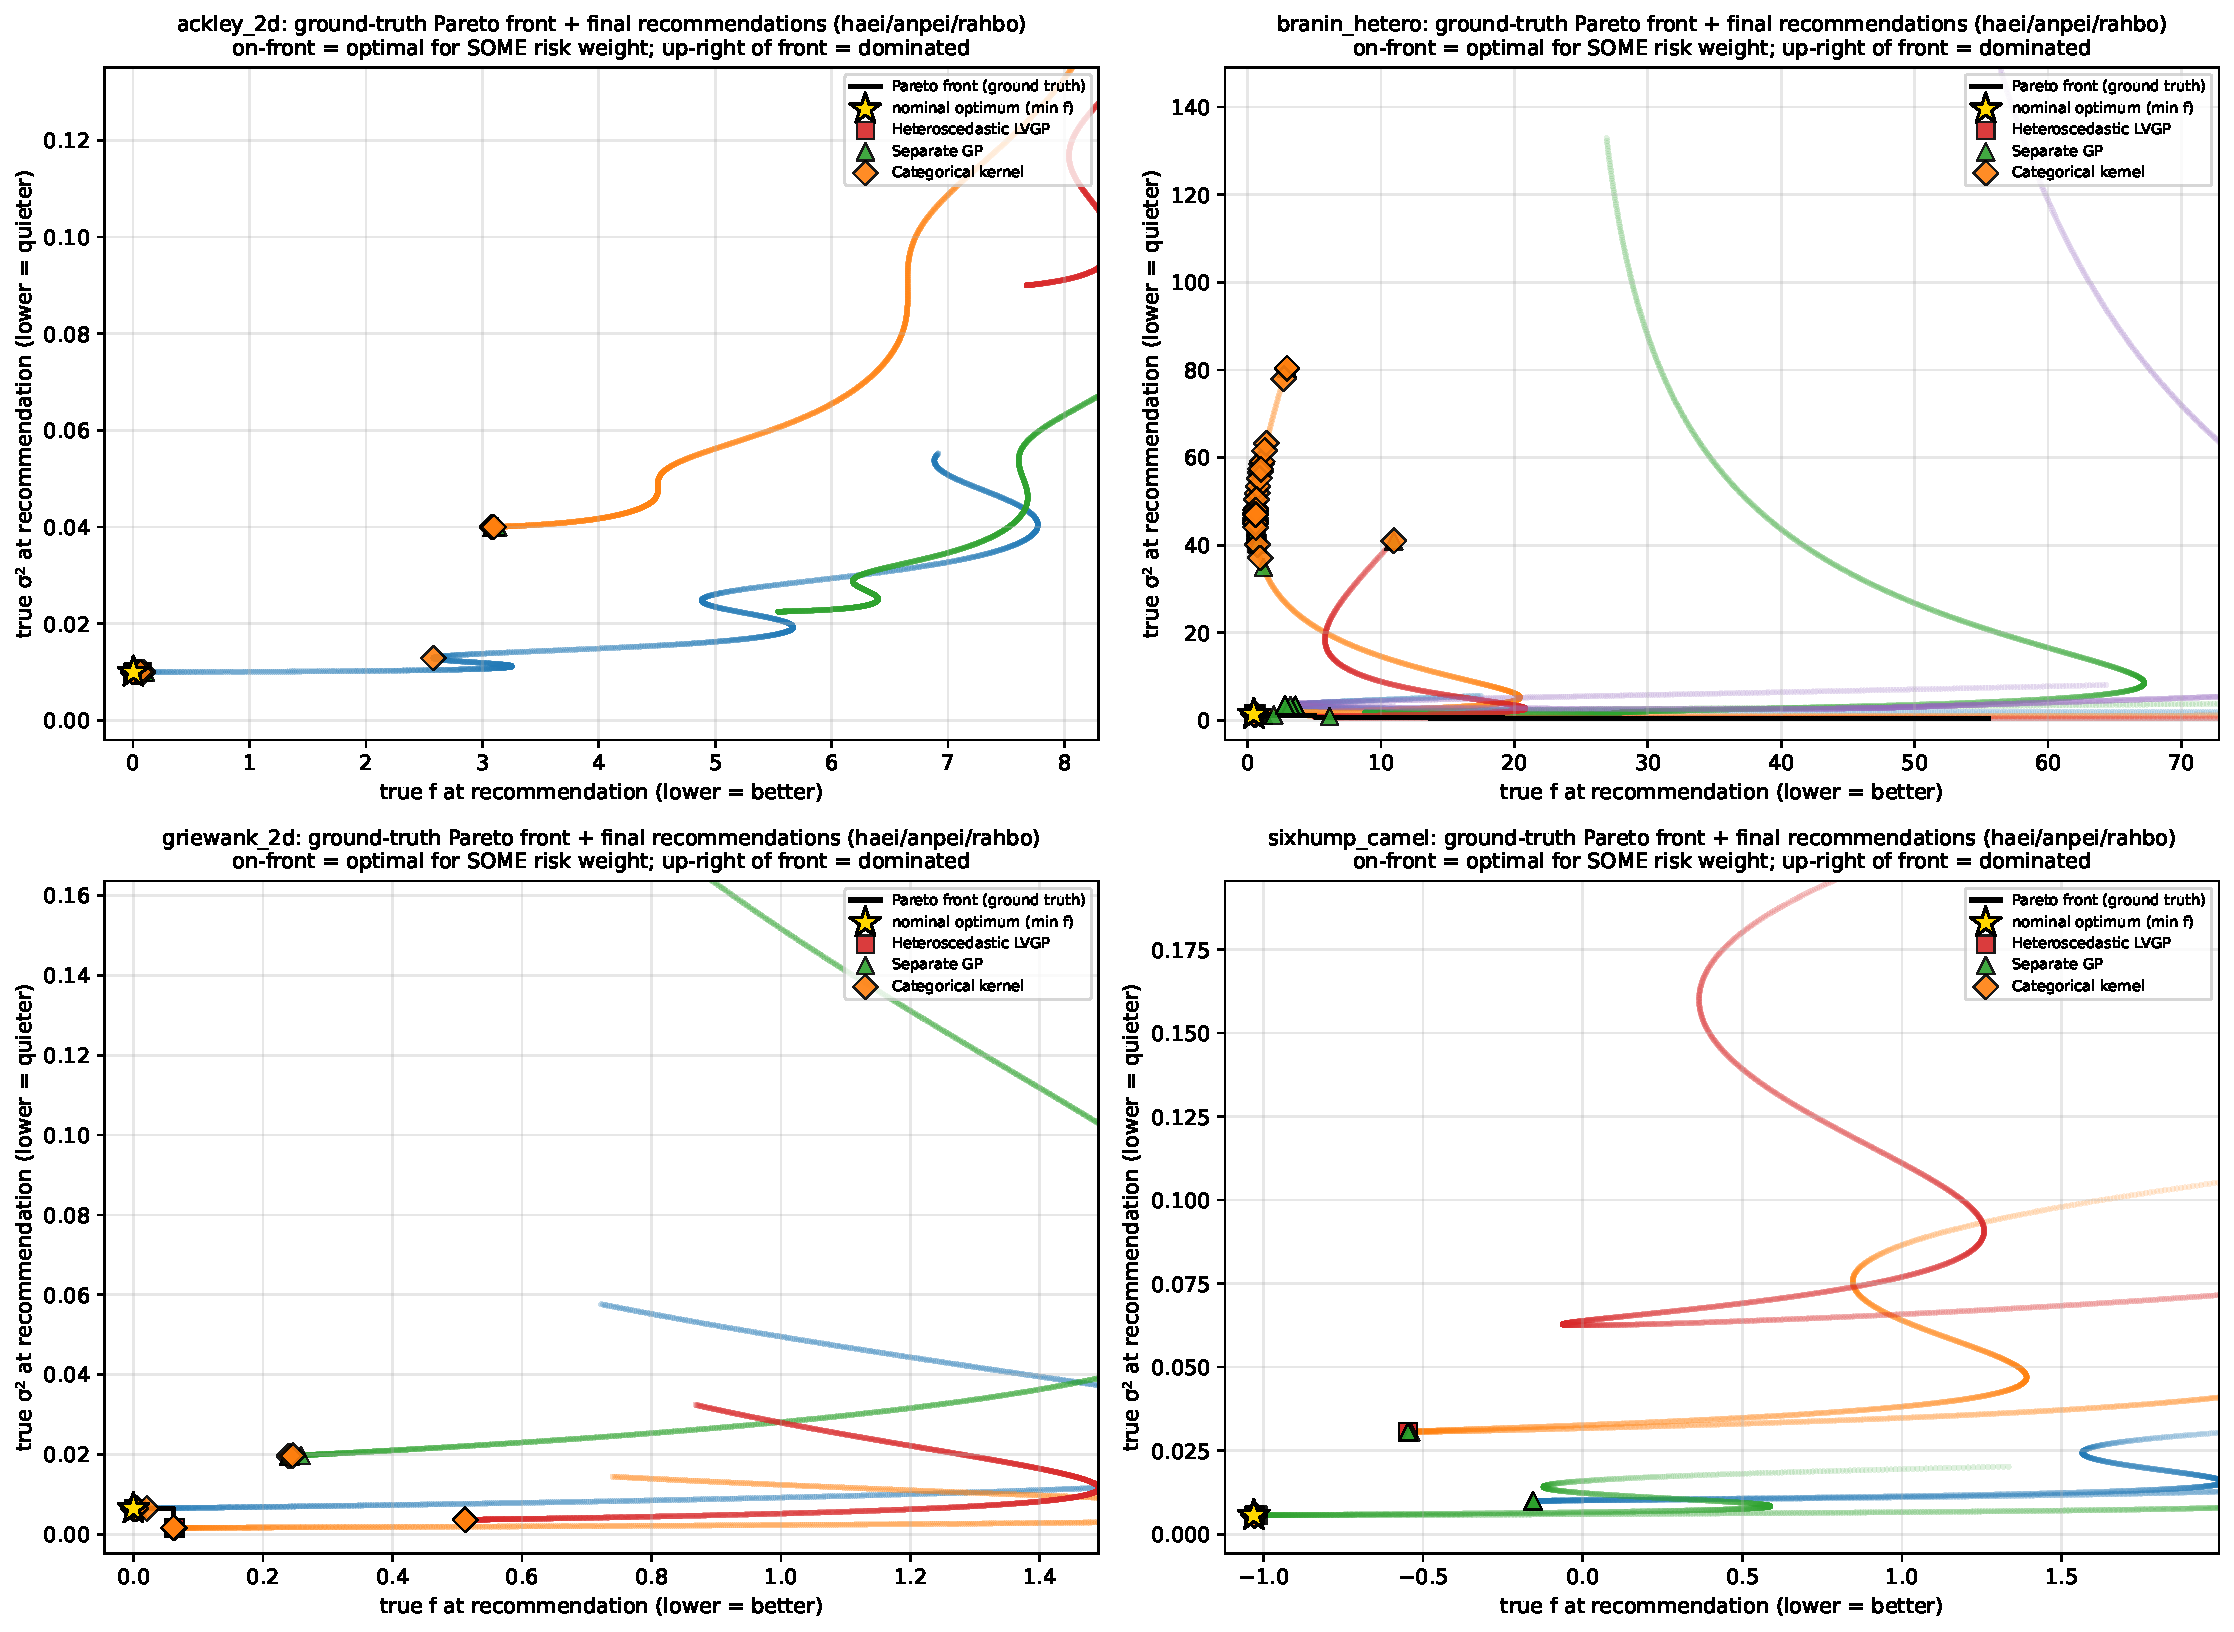
\includegraphics[width=0.78\textwidth]{figs/pareto_1d.pdf}
\caption{Hyperparameter-free view: ground-truth $(f,\sigma^2)$ Pareto front per 1-D problem,
with each model's final noise-aware recommendations overlaid. On-front = optimal for some
risk weight; up-right = dominated.}
\end{figure}

\finding{
(1) \textbf{The branin trap catches the categorical-kernel GP}: a cluster of its noise-aware
recommendations sits on the noisy twin ($\sigma^2 \approx 40$--$80$, dominated), while the
heteroscedastic LVGP's recommendations sit on the Pareto front near the quiet optimum.
(2) Only 3 of the 8 completed problems (branin, griewank\_2d, golinski) can discriminate
robust from non-robust methods; camel/ackley confirm no method is penalized when robustness
is free.
(3) At the sweep's $\alpha=0.5$ the robust and nominal optima coincide everywhere, so the MV
tables below ($\alpha=1$) largely mirror the regret tables; the discriminating comparison is
the pending $\alpha\in\{5,15\}$ sweep.}

\clearpage
\input{mv_nrep10_1d.tex}
\clearpage
\begin{table}[htbp]
\centering
\small
\setlength{\tabcolsep}{4pt}
\setlength{\fboxsep}{2pt}
\caption{Final mean-variance regret (RAHBO robustness, $\mathrm{MV}=f+\alpha\sigma^2$, $\alpha=1$) for every acquisition $\times$ surrogate model ($n_{\mathrm{rep}}=10$, mean $\pm$ sd over seeds).}
\label{tab:mv_nrep10}
\begin{tabular}{llrrrr}
\toprule
Acquisition & Model & Golinski & OTL Circuit & Piston & Rastrigin 6-D \\
\midrule
LCB & Standard LVGP & $3.48{\times}10^{-6} \pm 1.1{\times}10^{-7}$ & $3.87{\times}10^{-6} \pm 3.2{\times}10^{-6}$ & \colorbox{green!20}{{\boldmath$2.16{\times}10^{-7} \pm 1.5{\times}10^{-7}$}} & $29.2 \pm 7.3$ \\
 & Heteroscedastic LVGP & $1.72{\times}10^{-7} \pm 1.8{\times}10^{-9}$ & $4.64{\times}10^{-7} \pm 3.8{\times}10^{-7}$ & $4.6{\times}10^{-7} \pm 5.1{\times}10^{-7}$ & $25.1 \pm 5.7$ \\
 & Separate GP & \colorbox{green!20}{{\boldmath$0 \pm 0$}} & $0.00188 \pm 0.0038$ & $0.00098 \pm 0.00066$ & $19.2 \pm 11$ \\
 & Categorical kernel & \colorbox{green!20}{{\boldmath$0 \pm 0$}} & \colorbox{green!20}{{\boldmath$0 \pm 0$}} & $0.00102 \pm 0.00023$ & {\boldmath$6.53 \pm 4.3$} \\
\midrule
PI & Standard LVGP & $72.5 \pm 0$ & $0.056 \pm 0.029$ & $0.00122 \pm 0.00051$ & $20.7 \pm 6.8$ \\
 & Heteroscedastic LVGP & $1.37 \pm 2.6$ & $0.00586 \pm 0.0099$ & {\boldmath$2.93{\times}10^{-5} \pm 3.7{\times}10^{-5}$} & $23.5 \pm 3.1$ \\
 & Separate GP & \colorbox{green!20}{{\boldmath$0 \pm 0$}} & {\boldmath$6.94{\times}10^{-5} \pm 7{\times}10^{-5}$} & $0.000517 \pm 0.00037$ & $13.7 \pm 3.8$ \\
 & Categorical kernel & \colorbox{green!20}{{\boldmath$0 \pm 0$}} & $0.0159 \pm 0.011$ & $0.00119 \pm 0.0011$ & \colorbox{green!20}{{\boldmath$3.88 \pm 2.8$}} \\
\midrule
EI & Standard LVGP & $62.9 \pm 19$ & $0.0666 \pm 0.03$ & $0.0024 \pm 0.002$ & $32.5 \pm 11$ \\
 & Heteroscedastic LVGP & $6.77{\times}10^{-5} \pm 8.2{\times}10^{-5}$ & $0.0124 \pm 0.014$ & $0.00106 \pm 0.00057$ & $31.4 \pm 2.6$ \\
 & Separate GP & \colorbox{green!20}{{\boldmath$0 \pm 0$}} & {\boldmath$3.07{\times}10^{-5} \pm 6.1{\times}10^{-5}$} & {\boldmath$0.00099 \pm 0.00074$} & $13.1 \pm 9.6$ \\
 & Categorical kernel & \colorbox{green!20}{{\boldmath$0 \pm 0$}} & $0.0163 \pm 0.014$ & $0.002 \pm 0.00056$ & {\boldmath$3.91 \pm 2.2$} \\
\midrule
HAEI ($\gamma=0.5$) & Heteroscedastic LVGP & $7.82 \pm 4.1$ & $0.0119 \pm 0.013$ & $0.00323 \pm 0.0018$ & $30.6 \pm 5$ \\
 & Separate GP & \colorbox{green!20}{{\boldmath$0 \pm 0$}} & {\boldmath$3.07{\times}10^{-5} \pm 6.1{\times}10^{-5}$} & {\boldmath$0.000791 \pm 0.00055$} & $9.43 \pm 2.5$ \\
 & Categorical kernel & \colorbox{green!20}{{\boldmath$0 \pm 0$}} & $0.0157 \pm 0.013$ & $0.00249 \pm 0.00091$ & {\boldmath$4.79 \pm 1.6$} \\
\midrule
ANPEI ($\beta=0.8$) & Heteroscedastic LVGP & $0.965 \pm 1.4$ & $0.00408 \pm 0.0075$ & {\boldmath$0.00165 \pm 0.0013$} & $24.3 \pm 5.9$ \\
 & Separate GP & \colorbox{green!20}{{\boldmath$0 \pm 0$}} & {\boldmath$0.000202 \pm 0.00037$} & $0.00203 \pm 0.00067$ & $12.7 \pm 3.5$ \\
 & Categorical kernel & \colorbox{green!20}{{\boldmath$0 \pm 0$}} & $0.0289 \pm 0.017$ & $0.00226 \pm 0.00077$ & {\boldmath$3.96 \pm 2$} \\
\midrule
RAHBO ($\alpha=0.5$) & Heteroscedastic LVGP & {\boldmath$2.72 \pm 2.4$} & $2.74{\times}10^{-7} \pm 1.7{\times}10^{-7}$ & {\boldmath$4.57{\times}10^{-7} \pm 5.5{\times}10^{-7}$} & $20.7 \pm 4.5$ \\
 & Separate GP & $28.8 \pm 51$ & $0.00188 \pm 0.0038$ & $0.00115 \pm 0.00057$ & $21.2 \pm 8.6$ \\
 & Categorical kernel & $10.6 \pm 4$ & \colorbox{green!20}{{\boldmath$0 \pm 0$}} & $0.000695 \pm 0.00033$ & {\boldmath$5.2 \pm 2.6$} \\
\bottomrule
\end{tabular}
\end{table}


\section*{Pointers}
\begin{itemize}
\item \texttt{notebooks/compare.ipynb} --- full analysis (9 parts): convergence facets,
      per-problem reports, latent spaces, acquisition tables, robustness visuals
      (MV/quantile landscapes, Pareto, percentiles), model-quality metrics, exports.
\item \texttt{notebooks/compare\_v2.ipynb} --- curated narrative with equations and dated
      observation notes.
\item \texttt{notebooks/compare\_matlab\_python.ipynb} --- MATLAB vs native-python LVGP
      validation (equivalence, computing time, latent match).
\end{itemize}

\end{document}
